\documentclass[../main.tex]{subfiles}

\begin{document}
\section{Introduction: the spectrum and its approximation}

The computation of spectra can be considered the 'fundamental problem of
operator theory' \parencite{arveson2002short}. The spectrum of an operator holds
the same key to the entire structure as eigenvalues do for linear algebra,
however (as often occurs when passing from the finite- to infinite-dimensional
case) the problem is less tractable for general operators. For practical
applications, it is often necessary to rely on numerical techniques and
approximate methods to locate the spectrum, but we will see that these have
their own problems.

Our focus will be on differential, discrete difference, and multiplication
operators. As a result, we will not generally assume that the operator is
bounded (many texts use `operator' to mean `bounded operator'). However, we will
focus mainly on Hilbert spaces, and assume that the operator has the properties
required for the spectrum and adjoint to exist and make sense - these properties
are subtle and will not be an excessive restriction (merely allowing us to avoid
fiddly arguments required to deal with pathological examples).

All numerical examples shown below were calculated using \texttt{specpol}, a
Python package written by the author. Please see Appendix
\ref{sec:numerical-note} for more details on the technical implementation.
\subsection{Spectra}

We must first define our quantity of interest: the spectrum of an operator.
\begin{definition}{\textbf{(Resolvent and spectrum)}}\index{resolvent}\index{spectrum}
  (Adapted from \parencite{edmunds2018spectral})
  Let $T$ be a linear operator on a Banach space.
  \begin{itemize}
  \item The resolvent of $T$ is the set 
    $\rho(T) := \{\eta \in \mathbb{C} : (T - \eta I)\text{ has a bounded inverse}\}$,
    where I is the identity
    operator. If it exists, we call its inverse $(T - \eta I)^{-1}$
    the `resolvent operator' for $\eta$ and $T$.
  \item The spectrum of $T$, denoted $\Spec(T)$,is
    $\mathbb{C} \setminus \rho(T)$, i.e. the set of all complex numbers $\lambda$
    such that the operator $(T - \lambda I)$ does not have a bounded inverse.
  \end{itemize}
\end{definition}

In the remainder of the text, the identity operator $I$ will be implicit in the
operator - i.e. we will simply write $(T - \lambda I)$ as $(T - \lambda)$.

We must keep this generality (rather than just defining eigenvalues of a linear
operator like we do for matrices) because in infinite dimensions, the failure of
invertibility can come about in a variety of ways. In finite-dimensional spaces,
the rank-nullity theorem asserts that if $(T - \lambda)$ is not invertible, then
it is not injective. As a result, $(T - \lambda)u = (T - \lambda)v$ for some $u
\neq v$; so $T(u - v) = \lambda(u-v)$, and thus any point in the spectrum is an
eigenvalue. The variety of ways in which invertibility can generally fail will
be explored in Section \ref{sec:ess-spec}.

We will find many of our physical examples to be self-adjoint. We will prove
later that if an operator is self-adjoint, then its spectrum lies entirely on
the real line; this makes it much more convenient to model, bound and calculate
a wide range of results.

\begin{definition}{\textbf{(Adjoint, symmetric, and self-adjoint operators)}}
(Adapted from \cite{hall2013quantum})
\index{adjoint operator}\index{symmetric operator}\index{self-adjoint operator}
  \begin{itemize}
  \item Let $T$ be an operator on a Hilbert space $\hilbert$. Let $\Dom(T^*)$ be
    the set of all $v \in \hilbert$ such that the functional
	    $$u \mapsto (Tu, v) \quad \text{on $u \in \Dom(T)$}$$
    is bounded. We then define an \textbf{adjoint} operator $T^*$ to be the
    operator such that 
    $(Tu, v) = (u, T^*v)$ for all $u \in \Dom(T), v \in \Dom(T^*)$ 
  \item An operator $T$ is symmetric if 
    for all $u, v \in \Dom(T)$, (Tu, v) = (u, Tv).
  \item An operator $T$ is self-adjoint if it is symmetric and $Dom(T^*) =
    Dom(T)$, i.e. it is equal to its adjoint operator.
  \end{itemize}
\end{definition}

Note that a bounded operator is symmetric if and only if it is self-adjoint;
bounded operators are defined on the whole of $\hilbert$, so these issues with
the domain do not occur. 

As we have alluded to, there is no universal algorithm for the calculation of
operator spectra in the way that there is the QR algorithm
\cite{suli2003introduction} for matrices. To devise a formula for the spectrum
of even a specific subset of a class of operators is a mathematical feat, and
varieties of operators important to fields such as quantum physics
(\cite{lewin2010spectral}), hydrodynamics (\cite{manning2008descriptor}), and
crystallography (\cite{cances2012periodic}) still withhold the structure of
their spectra from decades-long attempts at discovery. 
To this end, we must employ numerical methods.
We shall find that even approximating spectra computationally is not so easy.

\subsection{Approximating spectra; Ritz and Galerkin methods}

It would be a reasonable hypothesis that we can approximate spectra by reducing
the infinite-dimensional problem to a finite-dimensional one, where we are on
much firmer ground when it comes to finding eigenvalues.

\begin{definition}{\textbf{(Compressions \& truncations)}}
(Adapted from \parencite{davies1995spectral})
\index{compression}\index{truncation}
  Let $T$ be an operator on a Hilbert space $\hilbert$, $\mathcal{L} \subseteq
  Dom(T)$ a closed linear subspace, and $P_\mathcal{L}$ the orthogonal
  projection of $\hilbert$ onto $\mathcal{L}$.
  \begin{itemize}
  \item The \textbf{compression} of the operator $T$, which we will often denote
    $T_\mathcal{L}$, is defined 
      $$T_\mathcal{L} \eqdef P_\mathcal{L} T\big|_{\mathcal{L}}$$
    where $\big|_{\mathcal{L}}$ denotes domain restriction to $\mathcal{L}$. 
  \item If $\{\phi_n\}_{n \in \mathbb{N}}$ is an orthonormal basis
    for $\hilbert$, the $k$'th \textbf{truncation} of $T$ is the compression
    of $T$ to $\text{Span}\{\phi_1, \phi_2, \hdots, \phi_k\}$. If
    there is no confusion, we will denote the k'th truncation $T_k$.
  \end{itemize}
\end{definition}

\begin{proposition}{\textbf{(Ritz matrix method)}}
\label{thm:ritz-method}
  The $k$'th truncation of an operator $T$ defined on the whole Hilbert space
  $\hilbert$ with orthonormal basis $\{\phi_n\}_{n \in \mathbb{N}}$ 
  is equivalently the matrix with entries
    $$T_{i,j} = (T\phi_i, \phi_j)$$
  for $i, j \in \{1, \hdots, k\}$.
  This matrix is known as the Ritz matrix of $T$ \cite{davies2003spectral}.
\end{proposition}
\begin{proof}
Take the subspace $\mathcal{L} = \text{Span}\{\phi_1, \phi_2, \hdots, \phi_k\}$ and
consider a solution
of the eigenvalue problem restricted to $\mathcal{L}$, that is, we want a function
$\tilde{u} \in \mathcal{L}$ such that $T\tilde{u} = \lambda\tilde{u}$; taking the inner
product on both sides, we get 
$(T\tilde{u}, \tilde{v}) = \lambda (\tilde{u}, \tilde{v})$ for all $\tilde{v}$
in $\mathcal{L}$. As any $\tilde{v}$ is a combination of basis functions, $\tilde{u}$
is a solution if and only if
$(T\tilde{u}, \phi_j) = \lambda (\tilde{u}, \phi_j)$ for all $j \in
\{1, \hdots, k\}$. Then as $\tilde{u} \in \mathcal{L},$ 
$$\tilde{u} = \sum_{i=1}^k u_i \phi_i$$
for some values $u_i$; if we substitute this into the problem we obtain a system
of linear equations:
\begin{align*}
  (T\tilde{u}, \phi_j) & = \sum_{i=1}^k (T\phi_i, \phi_j) u_i \\
  \lambda (\tilde{u}, \phi_j) & = \lambda u_j \\
  \Rightarrow \sum_{i=1}^k (T\phi_i, \phi_j) u_i & = \lambda u_j
\end{align*}

making use of the orthonormality of $\phi_i$ and $\phi_j$. This is equivalently
a matrix eigenvalue problem $M u = \lambda u$ where $M_{i,j} = (T\phi_i, \phi_j)$.
\end{proof}

One can use any sequence of truncations to finite-dimensional linear subspaces
to perform a Ritz approximation. For numerical approximation, using the span of
a subset of the orthonormal basis is a very suitable choice of subspace, as the
orthonormal basis functions can be enumerated and numerically evaluated with relative ease.

\begin{example}
Consider the right-shift operator $S$ on $\ell^2(\mathbb{N})$, which has the action
  $$Su_{n} = u_{n+1}.$$
We take the orthonormal basis $\phi_i(n) = \delta_{i, n}$ where $\delta$ is the Kronecker delta.
Then the 'infinite Ritz matrix' for $S$ is the matrix
  $$
    \begin{pmatrix*}[c]
      0 & 1 & 0 & 0 & \hdots \\
      0 & 0 & 1 & 0 & \hdots \\
      0 & 0 & 0 & 1 & \ddots \\
      \vdots & \vdots & \vdots & \ddots & \ddots \\ 
    \end{pmatrix*}
  $$
which we can truncate to approximate the spectrum of $S$.
\end{example}
Note if we were discussing $S$ on $\ell^2(\mathbb{Z})$, we would need the Ritz matrix to 'go in
both directions':
  $$
    \begin{pmatrix*}[c]
      \ddots & \ddots & & & \\ 
      \ddots & 0 & 1 & 0 & \\
       & 0 & 0 & 1 & 0 & \\
       & & 0 & 0 & 1 & \ddots \\
       & & & & \ddots & \ddots \\ 
    \end{pmatrix*}
  $$
taking care to not take this matrix 'too formally' (as the main diagonal is not well-defined
for a na\"ively defined bi-infinite matrix \cite{lindner2013where}). In these cases, it is
a natural choice to take the subspaces 
$\mathcal{L} = \text{Span}\{\phi_{-k}, \phi_{-k+1}, \hdots, \phi_{k-1} \phi_k\}$, 
intuitively 'cutting out the middle' of the bi-infinite matrix.

In the case of differential operators, we use a modified method
known as a Galerkin method; we will motivate and
explain the method via constructing an approximation method for a
one-dimensional Sturm-Liouville operator\index{Sturm-Liouville operator},
analogously to the Galerkin method for solving general symmetric second-order
PDEs given in \cite{suli2003introduction} and \cite{pryce1993numerical}. 

The one-dimensional Sturm-Liouville operator is

$$Lu = - \frac{d}{dx}(P(x)\frac{du}{dx}) + Q(x)u$$ 

which gives rise to the Sturm-Liouville eigenvalue problem with general boundary
conditions\footnote{See that the general boundary conditions cover the `regular'
set of homogeneous boundary conditions; Dirichlet if $a_2 = 0$, Neumann if $a_1
= 0$, Robin otherwise.}:

\begin{equation*}\label{eqn:sturm-liouville}
\tag{S-L}
\begin{cases}
Lu = \lambda u$$ \\
a_1 u(a) = a_2 u'(a), \ b_1 u(b) = b_2 u'(b)
\end{cases}
\end{equation*}

on a suitable subspace of $L^2[a, b]$, where $P$ and $Q$ are scalar-valued
functions. $Q$ is often called the `potential' of the operator. These operators
occur frequently in partial differential equations; for example, both the heat
and wave equations are governed by Sturm-Liouville operators.

To start, we will weaken the problem - currently, $u$ is required to be
twice-differentiable. We multiply both sides by a `test' function $v$ in some
suitable space, and integrate both sides to obtain
\begin{equation}\label{eqn:weak-pde}
-[Pu'v]^b_a + \int_a^b P(x) u'(x) v'(x) + Q(x) u(x) v(x) dx = \lambda \int_a^b u(x) v(x) dx
\end{equation}
which we tidy up into the form 
$\mathcal{A}[u, v] = \lambda (u, v)$
where $\mathcal{A}$ is the bilinear form defined as the left side of
(\ref{eqn:weak-pde}). and $(\cdot, \cdot)$ is the natural scalar product on
$L^2$.

The boundary term nicely encodes the boundary conditions of the original
problem into the equation.\footnote{For most boundary conditions, one can
substitute $u'$ via the boundary condition; for Dirichlet boundary conditions,
we will require $v$ to be zero at the boundaries.} We call a function $u$ such
that $\mathcal{A}[u, v] = \lambda (u, v)$ for all test functions $v$ a `weak
solution' of problem (\ref{eqn:sturm-liouville}). Note that to create this weak
form, we do not even need $u$ to be differentiable once; it just needs to be
integrable by parts with a test function.

This provides our suitable subspace of $L^2[a, b]$ (a Sobolev space) which is of
course much larger than the space of twice-differentiable functions. We will not
discuss the theory of Sobolev spaces in detail, but it is easy to see by direct
calculation that if $u$ is a weak solution and also twice-differentiable, then
it is a strong solution (as we can reverse the operation done in
(\ref{eqn:weak-pde}) to recover the initial problem)
\cite{brezis2011functional}.

Notice that if $u$ is in the domain of $L$, we have $\mathcal{A}[u, v] = (Lu,
v)$. Indeed, we can follow a similar argument to the proof of Proposition \ref{thm:ritz-method}
by replacing $(Tu, v)$ with $\mathcal{A}[u, v]$ to get the same matrix form.

The following example shows that this method can be effective:

\begin{example}
\label{ex:schrodinger-ritz}
Consider the following Schr\"odinger operator, which describes the movement of a
hydrogen atom's electron
\cite{pryce1993numerical}:\index{Schr\"odinger operator}

$$Hu = -u'' + (-\frac{1}{x} + \frac{2}{x^2})u$$
\end{example}

The spectrum of this operator, fascinatingly, corresponds to the energy levels
of certain `stable' states of the atom in quantum mechanics. The analysis of
this operator for larger atoms is an open problem; for example,
the spectrum for the equivalent equation in the helium atom (let alone any
larger atom!) has only been calculated numerically \cite{davies1995spectral}.
The hydrogen atom's spectrum can be found concretely, and in the space $L^2(0,
\infty)$ it has eigenvalues $\lambda_k = -\frac{1}{(2k + 4)^2}$ for $k \in
\mathbb{N}_0$.

Let us see how well a Ritz-Galerkin method can approximate this known spectrum.
We can see the results of an approximation in Figure \ref{fig:schrodinger-ritz}
done via the \texttt{specpol} software. We choose the weighted Laguerre
polynomial basis $\phi_n = \exp(-x/2)L_n$, where $L_n$ is the n'th Laguerre
polynomial; this is a complete orthonormal set on the half-line
\cite{szego1975orthogonal}. In this case, at a matrix size of 100, the 4
smallest eigenvalues are accurate to 3 significant figures (and despite possible
error induced via other numerical parts of the computation, e.g. inaccuracy in
the calculation of basis functions or in the quadrature used).

\pagebreak
\hspace{0pt}
\vfill
\begin{center}
\begin{figure}[h!]
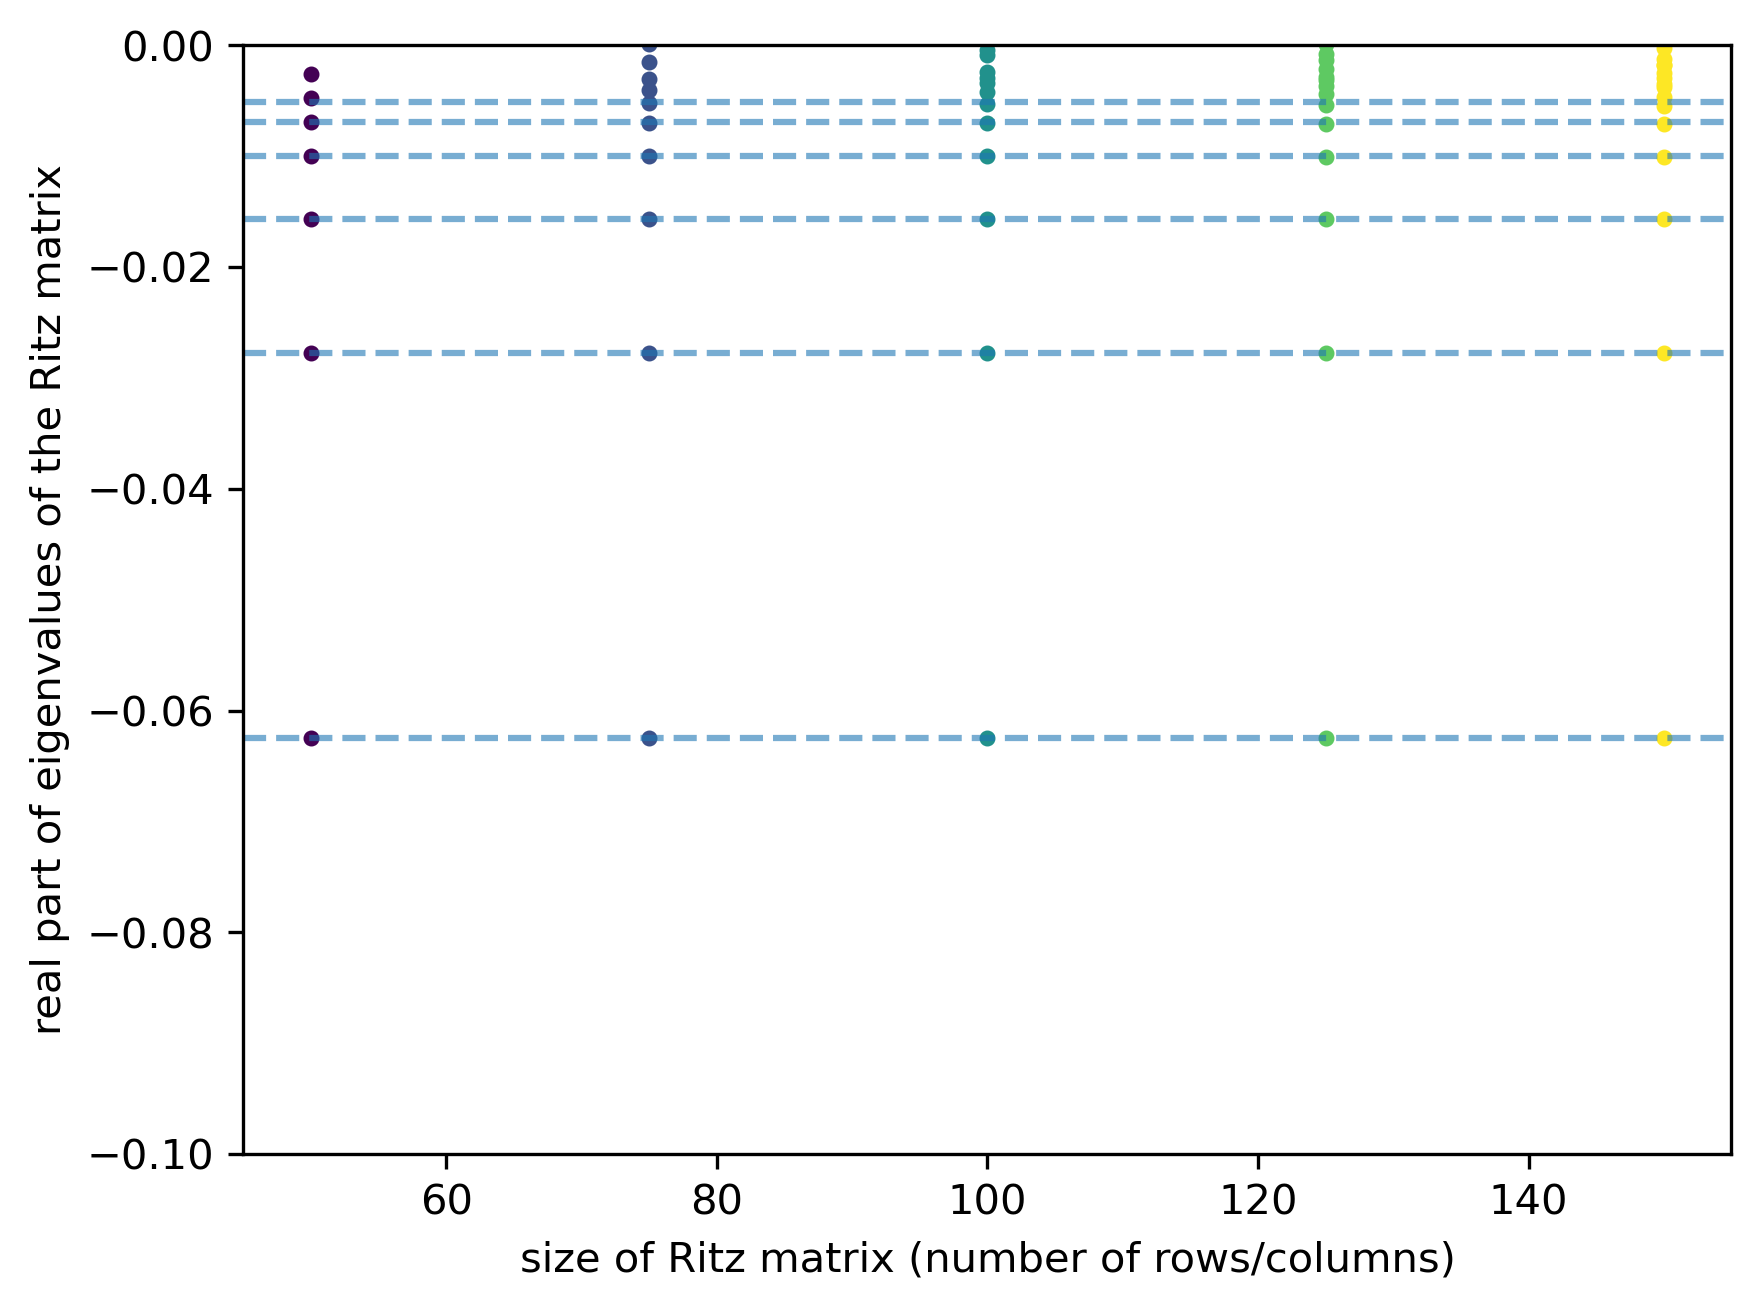
\includegraphics{hydrogen}
\caption{A Ritz-Galerkin approximation for the Schr\"odinger operator given
	above, cropped to ignore the positive spectrum (which is known to be the
	whole positive half-axis). The dotted lines correspond to where the
	first 6 eigenvalues should be according to the formula. Note how as the
	size of the Ritz matrix increases, the higher eigenvalues (closer to the
	origin, as they are a sequence converging to 0) `fill
	in'.}
	\label{fig:schrodinger-ritz}
\end{figure}
\begin{tabular}{c|c c}
 Eigenvalue & Exact & Approximated, rounded to 5sf \\
 \hline\hline
 $\lambda_0$ & -0.0625 & -0.062500$^\dag$\\
 $\lambda_1$ & -0.02\.7 &  -0.027777$^\ddag$\\
 $\lambda_2$ & -0.015625 & -0.15625(03)\\
 $\lambda_3$ & -0.01 & -0.010015 \\
 $\lambda_4$ & -0.0069\.4 & -0.0069974 \\
 $\lambda_5$ & $-0.00510204\hdots$ & -0.0052774\\
 \end{tabular}\\
 \quad\\
 Values for the first six lowest eigenvalues of the Ritz-Galerkin approxmiation for the
	hydrogen atom equation, at a matrix size of 100.
 \quad\\
 $\dag$: value to more significant figures is -0.06249999999978248, which was rounded to -0.0625 \\
 $\ddag$: value to more significant figures is -0.027777777778024638 \\
\end{center}
\vfill
\hspace{0pt}
\pagebreak

Indeed, comparing this derivation to the earlier definitions of truncations, we
can see that we are calculating the eigenvalues of truncations $T_n$ of the
operator $T$. The natural question which follows is to ask about the convergence
of these methods as $n$ becomes large. The answer is that this
convergence is not perfect - in fact,  for Schr\"odinger operators in particular
it has been shown that a `perfect' truncation algorithm is impossible
\cite{colbrook2019how}. In our case, the spectrum of the operator will be
approximated, but in many cases there will also be a lot of other spurious
values in the spectrum.

This brings us to our main subject; the study of these spurious eigenvalues, known as spectral pollution.

\subsection{Spectral pollution}

\begin{definition}{\textbf{(Spectral pollution)}}
(Adapted from \parencite{davies1995spectral})
\index{spectral pollution}
Let $(T_n)_{n \in \mathbb{N}}$ be an increasing sequence of truncations of an
operator $T$. A value $\lambda \in \mathbb{C}$ is said to be a point of
\textbf{spectral pollution} if there is a sequence $\lambda_n \in \Spec(T_n)$
such that $\lambda_n \rightarrow \lambda$ but $\lambda \notin \Spec(T)$.
\end{definition}

Points of spectral pollution are, intuitively, artefacts of an approximation
which will never converge to a point in the actual spectrum. We will see that
they exist for many types of operator, 
that they are relatively common, and that they may \emph{get worse} as
the approximation goes to higher iterations. Unless we already know what the
spectrum of the operator is, it can be incredibly hard for us to decide whether
a point is actually in the spectrum or whether it is
spurious. In applications of spectral theory, this difference can be beyond a
simple 'noisy data' nuisance - rather, a confounding problem, as we will see
in examples throughout.

Note that spectral pollution is caused by a variety of the 'moving parts' of
an approximation: for example, pollution can be introduced by a poor choice
of boundary condition \cite{cances2012periodic}, a truncation of the domain
\cite{aceto2006numerical}, or the choice of subspaces \cite{levitin2002spectral}.
One can easily intuit why the latter will affect the amount of pollution; it is
obvious that if we chose the eigenfunctions of the operator as our orthonormal basis,
then we would not have pollution (as our approximating matrices would be diagonal)
but for a different basis, the Ritz matrix may well be dense and complicated. Indeed,
some methods of avoiding pollution (e.g. \cite{boffi1999pollution}) rely on making
a deft choice of approximating spaces.

There are, of course, other methods for approximating operator spectra, such as
the popular finite difference or `shooting' methods \cite{suli2003introduction},
or specialised methods such as Pr\"ufer and Pruess methods for Sturm-Liouville
problems \cite{pryce1993numerical}, which are not subject to pollution. So why
do we care about truncation methods?

Firstly, many of the methods for approximating operator spectra will discover eigenvalues
in order. But for many operators, the spectrum contains continuous 'bands' of spectrum;
then the spectrum is uncountable, so these iterative methods will be 'stuck' at these
bands forever. Methods that 'globally' approximate spectra are few and far between
\cite{pryce1993numerical}.

Secondly, the central motivation for these methods is that they make \emph{almost no}
assumptions about the operator itself or the location of its spectrum. Even for
the operators covered by these specialised methods, eigenvalues in certain parts
of the spectrum cannot be accessed without significant tweaking
\cite{aceto2006numerical}, not to mention that many methods only apply to
problems in one dimension. If the spectral pollution for a sequence of
truncations can be discarded, detected or otherwise dealt with, it would provide
a unified and powerful approach to numerical spectral theory for almost any operator.
\end{document}
